\section{Exact two-branch structure}\label{sec:geometry}

\paragraph{Conventions.}
$\mathbb T=\mathbb R/2\pi\mathbb Z$ with the normalized measure $d\varphi/2\pi$. For $F\in L^1(\mathbb T)$ put
$\hat F(k)=\int_{\mathbb T}F(\varphi)e^{-ik\varphi}\,\tfrac{d\varphi}{2\pi}$, so that translating $F$ by $\tau$ multiplies $\hat F(k)$ by $e^{-ik\tau}$.
Points of the disk are written $z=re^{i\varphi}$, and $q(r)=\sqrt{r^2-a^2}$.
Fix $\varepsilon\in(0,(1-a)/3)$, put $I_\varepsilon=[a+\varepsilon,1-\varepsilon]$, $w=c/N$ and
$\tau_\varepsilon=\min(\varepsilon/2,a/2)$. Let $N_0=N_0(\varepsilon,c)$ be such that for $N\ge N_0$
\begin{equation}\label{deph:N0}
w<\tau_\varepsilon\qquad\text{and}\qquad (1-\varepsilon)^2-(a-w)^2<Q^2 ;
\end{equation}
the second condition holds for small $w$ because $(1-\varepsilon)^2-a^2<1-a^2=Q^2$. (Only $w<\min(\varepsilon/2,a)$ is needed
for Lemma~\ref{lem:branches}; the factor $1/2$ in front of $a$ is used in Lemma~\ref{deph:reg}.)
All $N$ below satisfy $N\ge N_0$.

\begin{figure}[t]
\centering
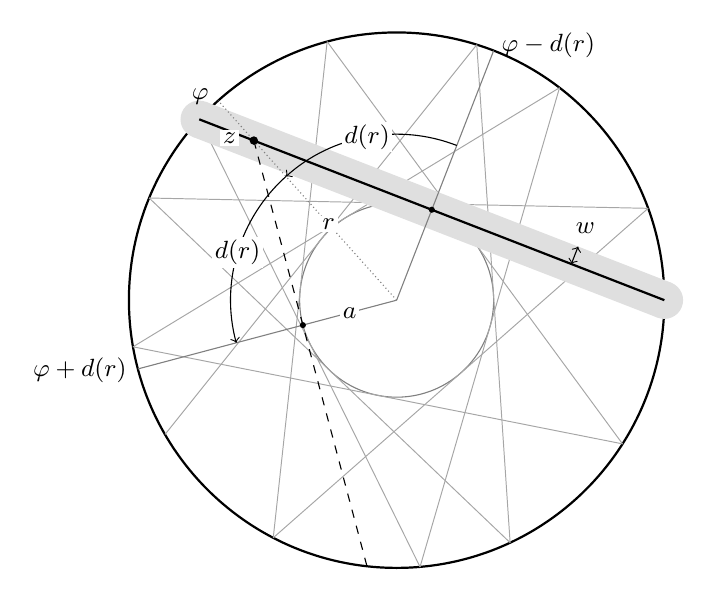
\begin{tikzpicture}[scale=0.85]
% CAPTION (for \caption in sections/dephasing.tex): Unit disk with the caustic circle of radius a = cos(alpha)
% (golden alpha), twelve chords of the orbit, and a point z at radius r > a. The two tangent lines from z to the caustic
% touch it in the directions phi -+ d(r), d(r) = arccos(a/r): the two angular branches. The solid chord lies on one branch;
% the dashed line is the other. The shaded stadium is the tube of half-width w around that chord (w exaggerated).
% generated by make_geometry.py; alpha=1.199982, a=0.362375, r=0.8, chord j=0
\draw[thick] (0,0) circle (4);
\draw[gray] (0,0) circle (1.4495);
\draw[gray!70, line width=0.35pt] (-2.9495,2.7020) -- (0.3497,-3.9847);
\draw[gray!70, line width=0.35pt] (0.3497,-3.9847) -- (2.4338,3.1744);
\draw[gray!70, line width=0.35pt] (2.4338,3.1744) -- (-3.9389,-0.6967);
\draw[gray!70, line width=0.35pt] (-3.9389,-0.6967) -- (3.3750,-2.1469);
\draw[gray!70, line width=0.35pt] (3.3750,-2.1469) -- (-1.0384,3.8629);
\draw[gray!70, line width=0.35pt] (-1.0384,3.8629) -- (-1.8436,-3.5498);
\draw[gray!70, line width=0.35pt] (-1.8436,-3.5498) -- (3.7573,1.3722);
\draw[gray!70, line width=0.35pt] (3.7573,1.3722) -- (-3.6974,1.5262);
\draw[gray!70, line width=0.35pt] (-3.6974,1.5262) -- (1.6954,-3.6229);
\draw[gray!70, line width=0.35pt] (1.6954,-3.6229) -- (1.1971,3.8167);
\draw[gray!70, line width=0.35pt] (1.1971,3.8167) -- (-3.4608,-2.0056);
\fill[gray!25] (4.1015,0.2610) -- (-2.8480,2.9629) -- (-3.0509,2.4410) -- (3.8985,-0.2610) -- cycle;
\fill[gray!25] (4.0000,0.0000) circle (0.2800); \fill[gray!25] (-2.9495,2.7020) circle (0.2800);
\draw[thick] (4.0000,0.0000) -- (-2.9495,2.7020);
\draw[dashed] (-2.1337,2.3848) -- (-0.4432,-3.9754);
\draw[gray] (0,0) -- (1.4495,3.7281);
\node[font=\small, inner sep=2pt, anchor=west] at (1.4785,3.8027) {$\varphi-d(r)$};
\draw[gray, densely dotted] (0,0) -- (-2.6671,2.9810);
\node[font=\small, inner sep=2pt, anchor=east] at (-2.7205,3.0406) {$\varphi$};
\draw[gray] (0,0) -- (-3.8658,-1.0275);
\node[font=\small, inner sep=2pt, anchor=east] at (-3.9431,-1.0481) {$\varphi+d(r)$};
\fill (0.5253,1.3510) circle (1.3pt);
\fill (-1.4009,-0.3724) circle (1.3pt);
\fill (-2.1337,2.3848) circle (1.8pt);
\node[font=\small, fill=white, inner sep=1pt] at (-2.4961,2.4248) {$z$};
\draw[->] (0.8987,2.3114) arc[start angle=68.754, end angle=131.820, radius=2.4800];
\draw[->] (-1.6536,1.8482) arc[start angle=131.820, end angle=194.885, radius=2.4800];
\node[font=\small, fill=white, inner sep=1pt] at (-0.4429,2.4401) {$d(r)$};
\node[font=\small, fill=white, inner sep=1pt] at (-2.3761,0.7105) {$d(r)$};
\node[font=\small, fill=white, inner sep=1pt] at (-0.7004,-0.1862) {$a$};
\node[font=\small, fill=white, inner sep=1pt] at (-1.0135,1.1328) {$r$};
\draw[<->, line width=0.4pt] (2.6101,0.5404) -- (2.7116,0.8014);
\node[font=\small, fill=white, inner sep=1pt] at (2.8203,1.0810) {$w$};

\end{tikzpicture}
\caption{Unit disk, caustic circle of radius $a=\cos\alpha$ (golden $\alpha$), twelve chords of the orbit, and a point
$z$ at radius $r>a$. The two tangent lines from $z$ to the caustic touch it in the directions $\varphi\mp d(r)$,
$d(r)=\arccos(a/r)$: these are the two angular branches. The solid chord lies on one branch, the dashed line is the other.
The shaded stadium is the tube of half-width $w$ about that chord ($w$ exaggerated).}
\label{deph:fig-geometry}
\end{figure}

\begin{lemma}\label{lem:branches}
For $r\in I_\varepsilon$ let $d_\mp(r)=\arccos((a\pm w)/r)$. A point $z=re^{i\varphi}$ satisfies
$\dist(z,\Gamma_N)\le w$ if and only if $\varphi-\theta_j\in\pm[d_-(r),d_+(r)]\pmod{2\pi}$ for some $j<N$.
\end{lemma}

\begin{proof}
Both $(a\pm w)/r$ lie in $(0,1)$: $a-w>0$ and $a+w<a+\varepsilon\le r$. So $0<d_-<d_+<\pi/2$.
Let $\delta=\varphi-\theta_j\in(-\pi,\pi]$. The distance from $z$ to the line $\mathbf n_j\cdot y=a$ is $|r\cos\delta-a|$, which is
at most $w$ iff $\cos\delta\in[(a-w)/r,(a+w)/r]$, i.e.\ iff $|\delta|\in[d_-,d_+]$ (this also excludes $|\delta|$ near $\pi$).
For such $\delta$, the coordinate of $z$ along the chord direction is $r|\sin\delta|\le r\sin d_+=\sqrt{r^2-(a-w)^2}<Q$
by \eqref{deph:N0}, while chord $j$ occupies the coordinates $[-Q,Q]$. So the foot of the perpendicular lies on the chord and
$\dist(z,[p_j,p_{j+1}])=\dist(z,\text{line}_j)\le w$. For other $\delta$ the distance to the chord is at least the distance to the
line, which exceeds $w$. Taking the minimum over $j<N$ gives the claim.
\end{proof}

Let $F_{N,s}$ be the indicator of the points of $\mathbb T$ at circular distance more than $s/N$ from every $\theta_j$, $j<N$; then
$\int F_{N,s}\,d\varphi/2\pi=m_N(s)$, $F_{N,s}$ is nonincreasing in $s$, and $\hat F_{N,s}(0)=m_N(s)$. Write
$\zeta(r,t)=\arccos((a+t)/r)$, so $d_\mp=\zeta(r,\pm w)$, and set
\[
\bar d_N=\tfrac12(d_++d_-),\quad h_N=\tfrac12(d_+-d_-),\quad s_N=Nh_N,\quad \psi_N=2\bar d_N=\zeta(r,w)+\zeta(r,-w).
\]
Since $\varphi-\theta_j\in[d_-,d_+]$ means $|\varphi-\bar d_N-\theta_j|\le h_N$, and likewise for the negative branch,
Lemma~\ref{lem:branches} says: $z$ is uncovered iff $F_{N,s_N(r)}(\varphi-\bar d_N)F_{N,s_N(r)}(\varphi+\bar d_N)=1$. Hence the
uncovered angular fraction at radius $r\in I_\varepsilon$ is
\begin{equation}\label{eq:autocorr}
U_N(r)=\int_{\mathbb T}F_{N,s_N(r)}(\varphi-\bar d_N)\,F_{N,s_N(r)}(\varphi+\bar d_N)\,\frac{d\varphi}{2\pi}=\mathcal C_{N,s_N(r)}(\psi_N(r)),
\end{equation}
with $\mathcal C_{N,s}(t)=\int F_{N,s}(\varphi)F_{N,s}(\varphi+t)\,d\varphi/2\pi$ (substitute $\varphi\mapsto\varphi+\bar d_N$).

\begin{lemma}\label{deph:reg}
There are constants $\Omega_\varepsilon,c_\varepsilon$ (depending on $a,\varepsilon,c$) such that for all $N\ge N_0$ and $r\in I_\varepsilon$:
\begin{enumerate}
\item $|s_N(r)-c/q(r)|\le c_\varepsilon/N$;
\item $\psi_N'(r)=\sum_\pm\dfrac{a\pm w}{r\sqrt{r^2-(a\pm w)^2}}\ \ge a$ and $|\psi_N''(r)|\le 2\Omega_\varepsilon$;
\item $\|\psi_N-\psi\|_{C^2(I_\varepsilon)}\le c_\varepsilon' /N^2$, where $\psi=2\arccos(a/r)$, $\psi'=2a/(rq)$.
\end{enumerate}
\end{lemma}

\begin{proof}
On $K=I_\varepsilon\times[-\tau_\varepsilon,\tau_\varepsilon]$ the argument $(a+t)/r$ lies in $[a/2,(a+\varepsilon/2)/(a+\varepsilon)]\subset(0,1)$, where $\arccos$
is real analytic. So $\zeta$ is real analytic near the compact set $K$, and every partial derivative of $\zeta$ is bounded on $K$;
let $\Omega_\varepsilon$ bound $|\partial_r^2\zeta|$, $|\partial_t^2\zeta|$, $|\partial_r^j\partial_t^2\zeta|$ ($j\le2$) on $K$. Explicitly,
$\partial_t\zeta=-(r^2-(a+t)^2)^{-1/2}$ and $\partial_r\zeta=(a+t)\,[r\sqrt{r^2-(a+t)^2}]^{-1}$.

(1) $s_N=\frac{N}{2}\bigl(\zeta(r,-w)-\zeta(r,w)\bigr)=\frac c{2w}\int_{-w}^{w}(-\partial_t\zeta)(r,t)\,dt$ is the mean of $-\partial_t\zeta$ over $[-w,w]$,
and $-\partial_t\zeta(r,0)=1/q(r)$. Since $|\partial_t\zeta(r,t)-\partial_t\zeta(r,0)|\le \Omega_\varepsilon|t|$, we get $|s_N-c/q|\le c\Omega_\varepsilon w=c^2\Omega_\varepsilon/N$.

(2) The formula is $\partial_r\zeta(r,w)+\partial_r\zeta(r,-w)$. Each term is at least $(a\pm w)/r^2\ge a/2$, because $\sqrt{r^2-(a\pm w)^2}\le r\le1$ and
$a\pm w\ge a/2$. The bound on $\psi_N''$ is $|\partial_r^2\zeta|\le \Omega_\varepsilon$ twice.

(3) $\psi_N-\psi=\zeta(r,w)+\zeta(r,-w)-2\zeta(r,0)=w^2\int_0^1(1-u)\bigl[\partial_t^2\zeta(r,uw)+\partial_t^2\zeta(r,-uw)\bigr]du$; differentiating
in $r$ up to twice under the integral gives the bound $2\Omega_\varepsilon w^2$.
\end{proof}

Only (1) and (2) are used below; (3) records the limiting lag $\psi=2\arccos(a/r)$.

\section{Proof of Theorem~\ref{thm:A}}\label{sec:proofA}

Write $\widetilde V_N=a^2+2\int_a^1r\,m_N(c/q(r))^2dr=a^2+2\int_0^Qq\,m_N(c/q)^2dq$ (substituting $q\,dq=r\,dr$).
Since $|\{z:|z|\in dr\}|=2\pi r\,dr$, $V_N=2\int_0^1rU_N(r)\,dr$ with $U_N(r)$ the uncovered fraction of the circle of radius $r$.
Fix $\varepsilon$, $N\ge N_0$.

\emph{Idea of the proof.} By Lemma~\ref{lem:branches} the uncovered fraction at radius $r$ is the autocorrelation $\mathcal C_{N,s}(\psi)$ of the circle vacancy indicator at lag $\psi_N(r)$. Its zero Fourier mode is $m_N(s)^2$. The nonzero modes die for two independent reasons: each coefficient $\hat F_{N,s}(k)$ tends to $0$ because the orbit is almost invariant under an irrational rotation (Step 1), and the lag moves with $r$ at speed bounded below, so oscillatory integrals gain a factor $1/|k|$ (Step 2). Steps 3 and 4 unfreeze $s$ and assemble the limits.

\emph{Step 0: layers.} Write $a^2=\int_0^a2r\,dr$, so $\widetilde V_N=\int_0^a2r\,dr+\int_a^12r\,m_N^2\,dr$, and compare piece by piece
using $0\le U_N,m_N\le1$.
\begin{itemize}
\item $r<a-w$: every line has distance $\ge a-r>w$ from $x$, so $U_N=1$; both sides contribute $(a-w)^2$. Difference $0$.
\item $r\in[a-w,a]$: $V_N$ contributes $\in[0,a^2-(a-w)^2]$, and $\widetilde V_N$ contributes exactly $a^2-(a-w)^2\le2aw\le2w$. Difference $\le2w$.
\item $r\in[a,a+\varepsilon]$: both contributions lie in $[0,(a+\varepsilon)^2-a^2]$, and $(a+\varepsilon)^2-a^2=\varepsilon(2a+\varepsilon)\le2\varepsilon$. Difference $\le2\varepsilon$.
\item $r\in[1-\varepsilon,1]$: both lie in $[0,1-(1-\varepsilon)^2]\subset[0,2\varepsilon]$. Difference $\le2\varepsilon$.
\end{itemize}
Therefore, with $w<\varepsilon/2$ (so that the total is also $\le6\varepsilon+2w$),
\begin{equation}\label{deph:layers}
|V_N-\widetilde V_N|\le4\varepsilon+2w+|\mathcal E_N|,\qquad
\mathcal E_N=\int_{I_\varepsilon}2r\bigl[\mathcal C_{N,s_N(r)}(\psi_N(r))-m_N(c/q(r))^2\bigr]dr .
\end{equation}

\emph{Step 1: low modes.} Rotation by $2\alpha$ maps $\{\theta_0,\dots,\theta_{N-1}\}$ to $\{\theta_1,\dots,\theta_N\}$, so
$F_{N,s}(\cdot-2\alpha)$ and $F_{N,s}$ differ only on the two closed arcs of half-length $s/N$ about $\theta_0$ and $\theta_N$ (overlaps
with other arcs only shrink the difference):
$\|F_{N,s}(\cdot-2\alpha)-F_{N,s}\|_{L^1(d\varphi/2\pi)}\le2s/(\pi N)$. Taking Fourier coefficients,
\[
|e^{-2ik\alpha}-1|\,|\hat F_{N,s}(k)|\le\frac{2s}{\pi N}\qquad(k\in\mathbb Z).
\]
Since $\beta=\alpha/\pi\notin\mathbb Q$, $e^{-2ik\alpha}=e^{-2\pi ik\beta}\ne1$ for $k\ne0$. Hence for every fixed $s\ge0$ and $k\ne0$,
$\hat F_{N,s}(k)\to0$ as $N\to\infty$. This is the only use of irrationality.

\emph{Step 2: high modes, frozen $s$.} $F_{N,s}$ is real with $F_{N,s}^2=F_{N,s}$, so Parseval gives $\sum_k|\hat F_{N,s}(k)|^2=m_N(s)\le1$ and
$\mathcal C_{N,s}(t)=\sum_k|\hat F_{N,s}(k)|^2e^{ikt}$, absolutely and uniformly convergent; the $k=0$ term is $m_N(s)^2$.
Let $J=[r_1,r_2]\subset I_\varepsilon$ and $k\ne0$. By Lemma~\ref{deph:reg}(2), $\psi_N'\ge a>0$, so integrating by parts,
\[
\int_J2r\,e^{ik\psi_N}dr=\Bigl[\frac{2r\,e^{ik\psi_N}}{ik\,\psi_N'}\Bigr]_{r_1}^{r_2}-\frac1{ik}\int_J\Bigl(\frac{2r}{\psi_N'}\Bigr)'e^{ik\psi_N}dr,
\]
and $|2r/\psi_N'|\le2/a$, $|(2r/\psi_N')'|=\bigl|2/\psi_N'-2r\psi_N''/\psi_N'^2\bigr|\le2/a+4\Omega_\varepsilon/a^2$. Since $|J|\le1$,
\begin{equation}\label{deph:ibp}
\Bigl|\int_J2r\,e^{ik\psi_N(r)}dr\Bigr|\le\frac{\mathcal B_\varepsilon}{|k|},\qquad \mathcal B_\varepsilon=\frac6a+\frac{4\Omega_\varepsilon}{a^2},
\end{equation}
uniformly in $N\ge N_0$, $J\subset I_\varepsilon$, $k\ne0$. Interchanging sum and integral, for every $s\ge0$ and $K\ge1$,
\begin{multline}\label{deph:frozen}
\Bigl|\int_J2r\bigl[\mathcal C_{N,s}(\psi_N(r))-m_N(s)^2\bigr]dr\Bigr|\le\sum_{0<|k|\le K}|\hat F_{N,s}(k)|^2+\mathcal B_\varepsilon\sum_{|k|>K}\frac{|\hat F_{N,s}(k)|^2}{|k|}\\
\le\sum_{0<|k|\le K}|\hat F_{N,s}(k)|^2+\frac{\mathcal B_\varepsilon}K,
\end{multline}
using $\int_J2r\,dr\le1$ for the low-frequency part. By Step 1 the finite sum tends to $0$ as $N\to\infty$ with $K,s$ fixed.

\emph{Step 3: unfreezing.} For $0\le s<t$ the sets $\{F_{N,s}=1\}$ and $\{F_{N,t}=1\}$ differ by at most $2N$ arcs of length $(t-s)/N$, so
$\|F_{N,s}-F_{N,t}\|_{L^1(d\varphi/2\pi)}\le(t-s)/\pi$. With $0\le F\le1$ this gives, uniformly in $N$ and in the lag,
\[
|\mathcal C_{N,s}(\cdot)-\mathcal C_{N,t}(\cdot)|\le\frac{2|s-t|}\pi,\qquad |m_N(s)^2-m_N(t)^2|\le\frac{2|s-t|}\pi .
\]
Fix $\eta>0$. As $r\mapsto c/q(r)$ is continuous on $I_\varepsilon$, choose a partition $I_\varepsilon=J_1\cup\dots\cup J_L$ into
intervals (with disjoint interiors) such that $c/q$ oscillates by less than $\eta$ on each $J_i$, and a value $s_i=c/q(r_i)$ with $r_i\in J_i$.
By Lemma~\ref{deph:reg}(1), $\sup_{I_\varepsilon}|s_N-c/q|<\eta$ for $N\ge N_1(\eta,\varepsilon)$. Then for $r\in J_i$, $|s_N(r)-s_i|<2\eta$ and $|c/q(r)-s_i|<\eta$, so
\[
\bigl|\mathcal C_{N,s_N(r)}(\psi_N)-m_N(c/q)^2-\bigl[\mathcal C_{N,s_i}(\psi_N)-m_N(s_i)^2\bigr]\bigr|\le\frac{4\eta}\pi+\frac{2\eta}\pi=\frac{6\eta}\pi .
\]
Integrating against $2r\,dr$ over $I_\varepsilon$ (total mass $\le1$) and applying \eqref{deph:frozen} on each $J_i$ with $s=s_i$:
\[
|\mathcal E_N|\le\frac{6\eta}\pi+\sum_{i=1}^L\Bigl[\sum_{0<|k|\le K}|\hat F_{N,s_i}(k)|^2+\frac{\mathcal B_\varepsilon}K\Bigr]
\qquad(N\ge\max(N_0,N_1)).
\]

\emph{Step 4: limits.} In the last display $\varepsilon,\eta$ (hence $L$ and the $s_i$) and $K$ are fixed; $L$ is finite, and
the finite sum of Fourier coefficients tends to $0$ as $N\to\infty$ by Step 1. Thus
$\limsup_N|\mathcal E_N|\le6\eta/\pi+L\mathcal B_\varepsilon/K$ for every $K$. Letting $K\to\infty$ and then $\eta\to0$
(note $L$ depends on $\eta$ but not on $K$) gives $\mathcal E_N\to0$. By \eqref{deph:layers}, and $w=c/N\to0$,
$\limsup_N|V_N-\widetilde V_N|\le4\varepsilon$ for each $\varepsilon\in(0,(1-a)/3)$, whence $V_N-\widetilde V_N\to0$.
This is Theorem~\ref{thm:A}. \qed

\begin{remark}
Order of limits: $\varepsilon$ fixed, then the partition ($\eta$, $L$, $s_i$), then the cutoff $K$; let $N\to\infty$, then
$K\to\infty$, then $\eta\to0$, and finally $\varepsilon\to0$. No rate is obtained: the rate in Step~1 depends on how well $k\beta$ is
approximated by integers, which is why only the qualitative statement is made.
\end{remark}
